\chapter{Overall understanding data and process BPIC 2017}
\\

\section{Case study}
Bank's loan process was proposed as case a study in BPIC 2017 from Dutch financial institute in The Netherlands. In such cases, certain problematic in the way how the process perform, process down time and interacting with client are challenging.
Precisely, the first question, the throughput times per part of the process,  in particular the difference between the time spent in the company's systems waiting for processing by a user and the time spent waiting on input from the applicant as this is currently unclear\cite{tue}.
In this thesis, we will consider submitted reports from the student category.
To understand the process presented in the challenge is it useful to structure the schema in mind as follow: An application is submitted. Then, some automatic checks are performed, then generate the suitable offer to client. This offer could be sent by online or by mail. A phone discussion then is made with client about this offer and waiting him/her to confirm the offer and send additional documents and information is needed. When receiving, a validation phase to assess offer is mandatory. In case of incomplete application or missing information, the financial institute will again contact the client to add them. When completion, A series of checks should be performed after which the verdict of application is made. A process as is following this logic considered in happy path.

\section{Dataset}
The dataset is a standard XES\footnote{} file extracted from ERP systems in the bank. For simple analysis this log we first used two process mining tools (Disco\footnote{https://fluxicon.com} and Celonis\footnote{https://www.celonis.com}). The log contains 31,509 application cases. By this, there are 561,671 events. Cases follow 4,047 variants (path) from begin to end.
There are 26 Activities, each can be in on of life cycle states (schedule, start, suspend, resume or ate abort).
There are 3 families of activities: 

Application state activities: ( A\_Create Application, A\_Submitted, A\_Concept,…)
Offer state activities: ( O\_Created, O\_Sent, O\_Accepted,…) and
Work item activities: ( W\_Call after offers, W\_Validate application, …)

We can also distinguish three classes of outcome as a final decision of any case:
A\_Pending, for accepting a loan request,
A\_Denied, for rejecting the loan request and
A\_Cancelled, to ignore the request by the client.

In addition, every case has other attributes, for instance, Loan goal, requested amount, resource, etc.. 


\section{Case study analysis}
Our area of interest is analysing case outcome probabilities regarding given information about the process. Using process mining tools and techniques we can derive more knowledge of how as-is business process performs and detect inefficiencies along the process. 
\\

Mining process regarding outcome: 
We show the three outcome classes by this log figure shows that we have about 17,000
Applications are positively decided, about 3,800 applications have been rejected after assessment and about 10,000 applications mentioned as cancelled figure \ref{fig:outcome}(A).
\\

Outcome mining regarding throughput time:
As a very useful dimension to work with process mining that it has several perspectives such as time perspective
To drill down for more clear view of causes, we aligned to view time perspective over the process. 
We can see a significant dependency on case period between 29-34 days and considering as cancellation of the request, this appears in 5,833 cases (19\% of all log) figure \ref{fig:outcome}(B) most of this time spent by waiting client to respond (i.e. sending needed documents for new offer or incomplete application) which is the case for 7,359 applications (23\% of log) figure \ref{fig:outcome}(C).
\\
\begin{figure}[h]
\centering
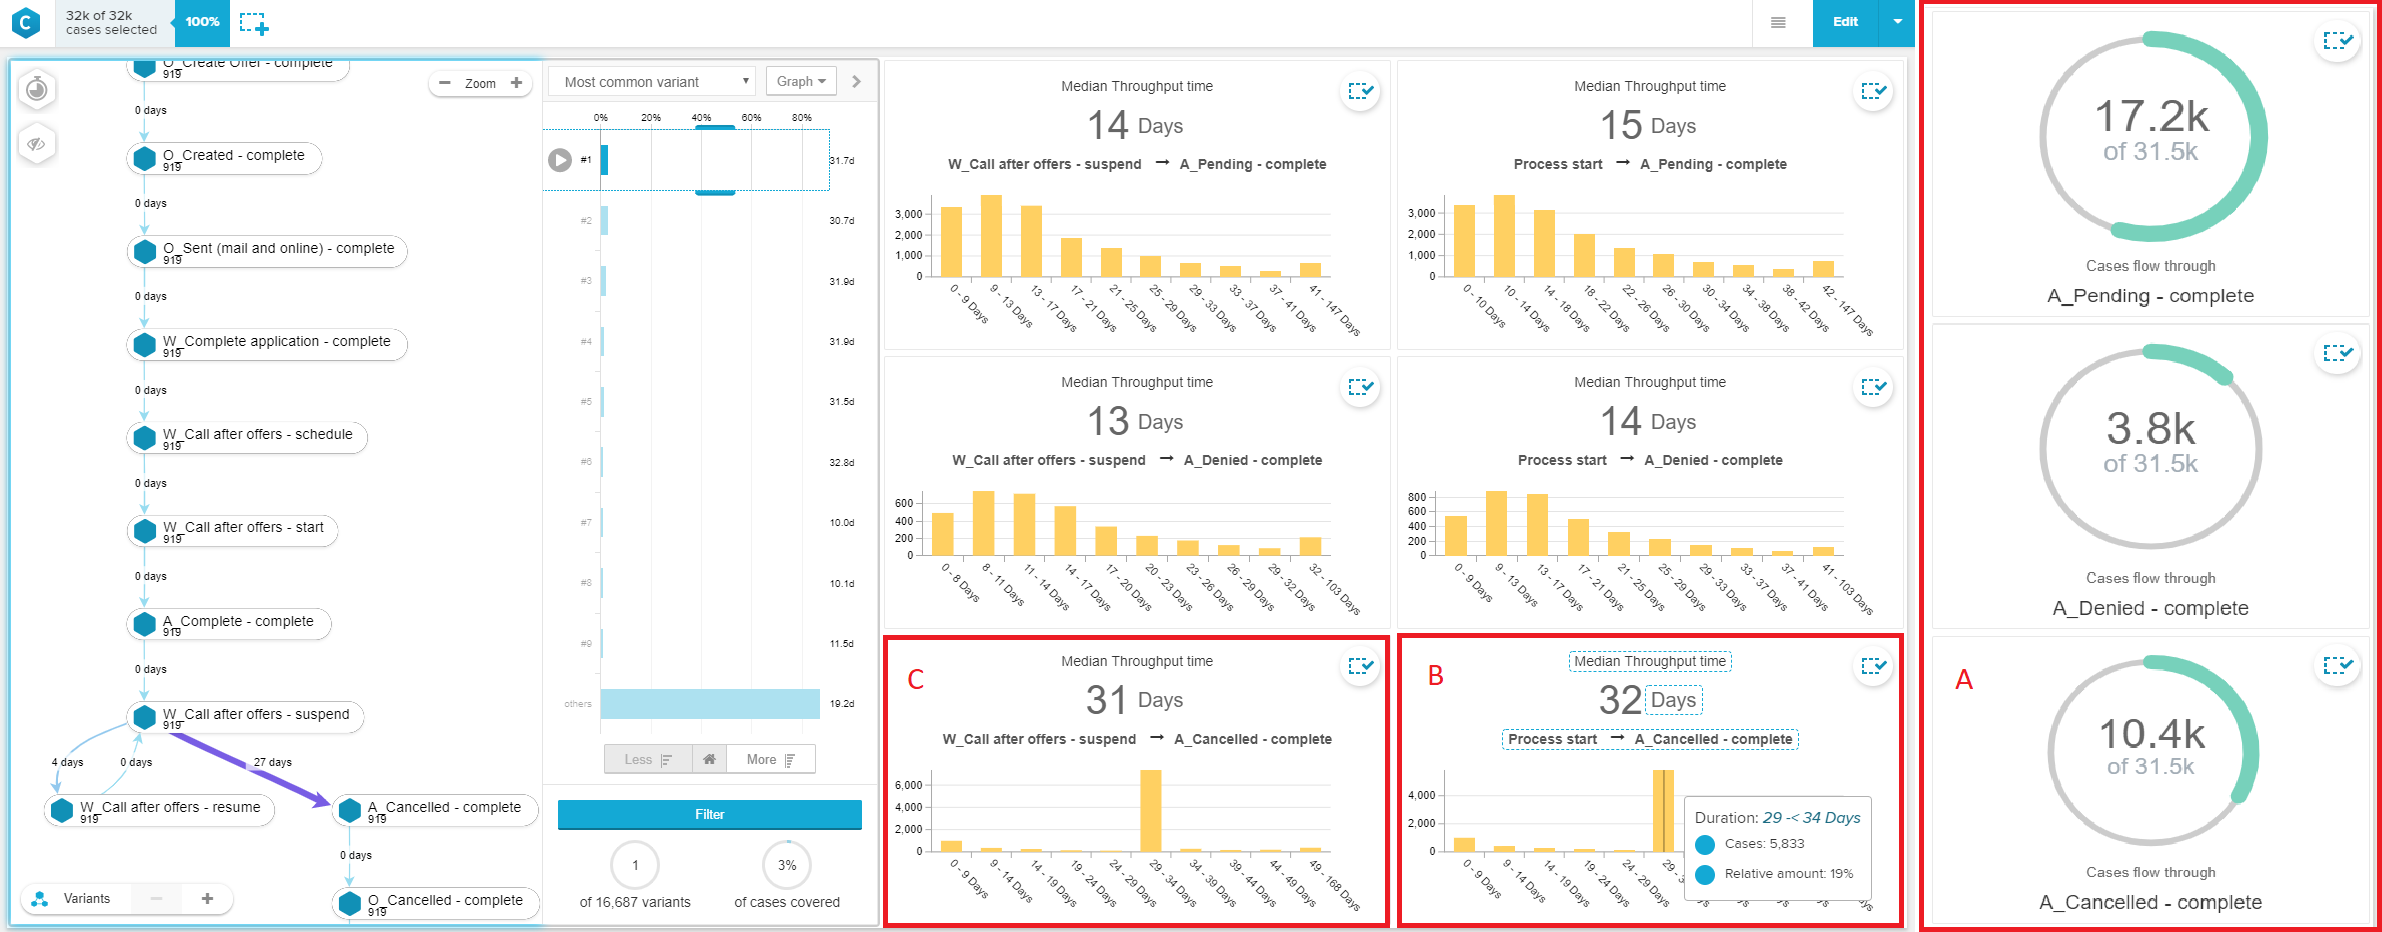
\includegraphics[width=\textwidth]{images/throughput_time.png}
\caption{\label{fig:outcome}Loan process mining in time perspective.}
\end{figure}

%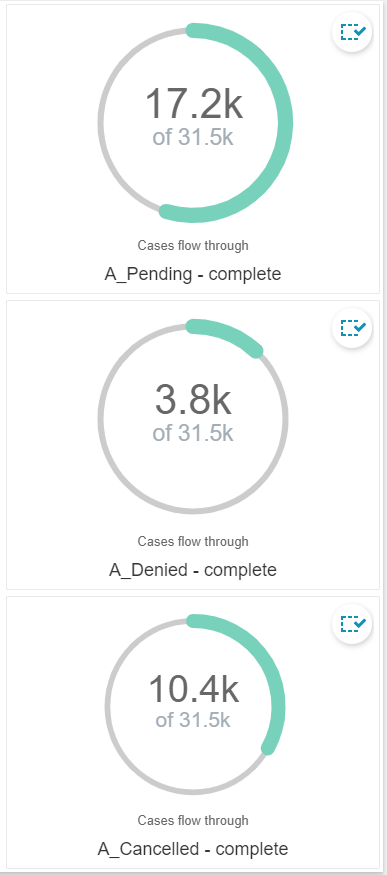
\includegraphics[width=5cm, height=10cm]{outcome}
%\begin{wrapfigure}{l}{0.9\textwidth} %this figure will be at the right
%\centering
%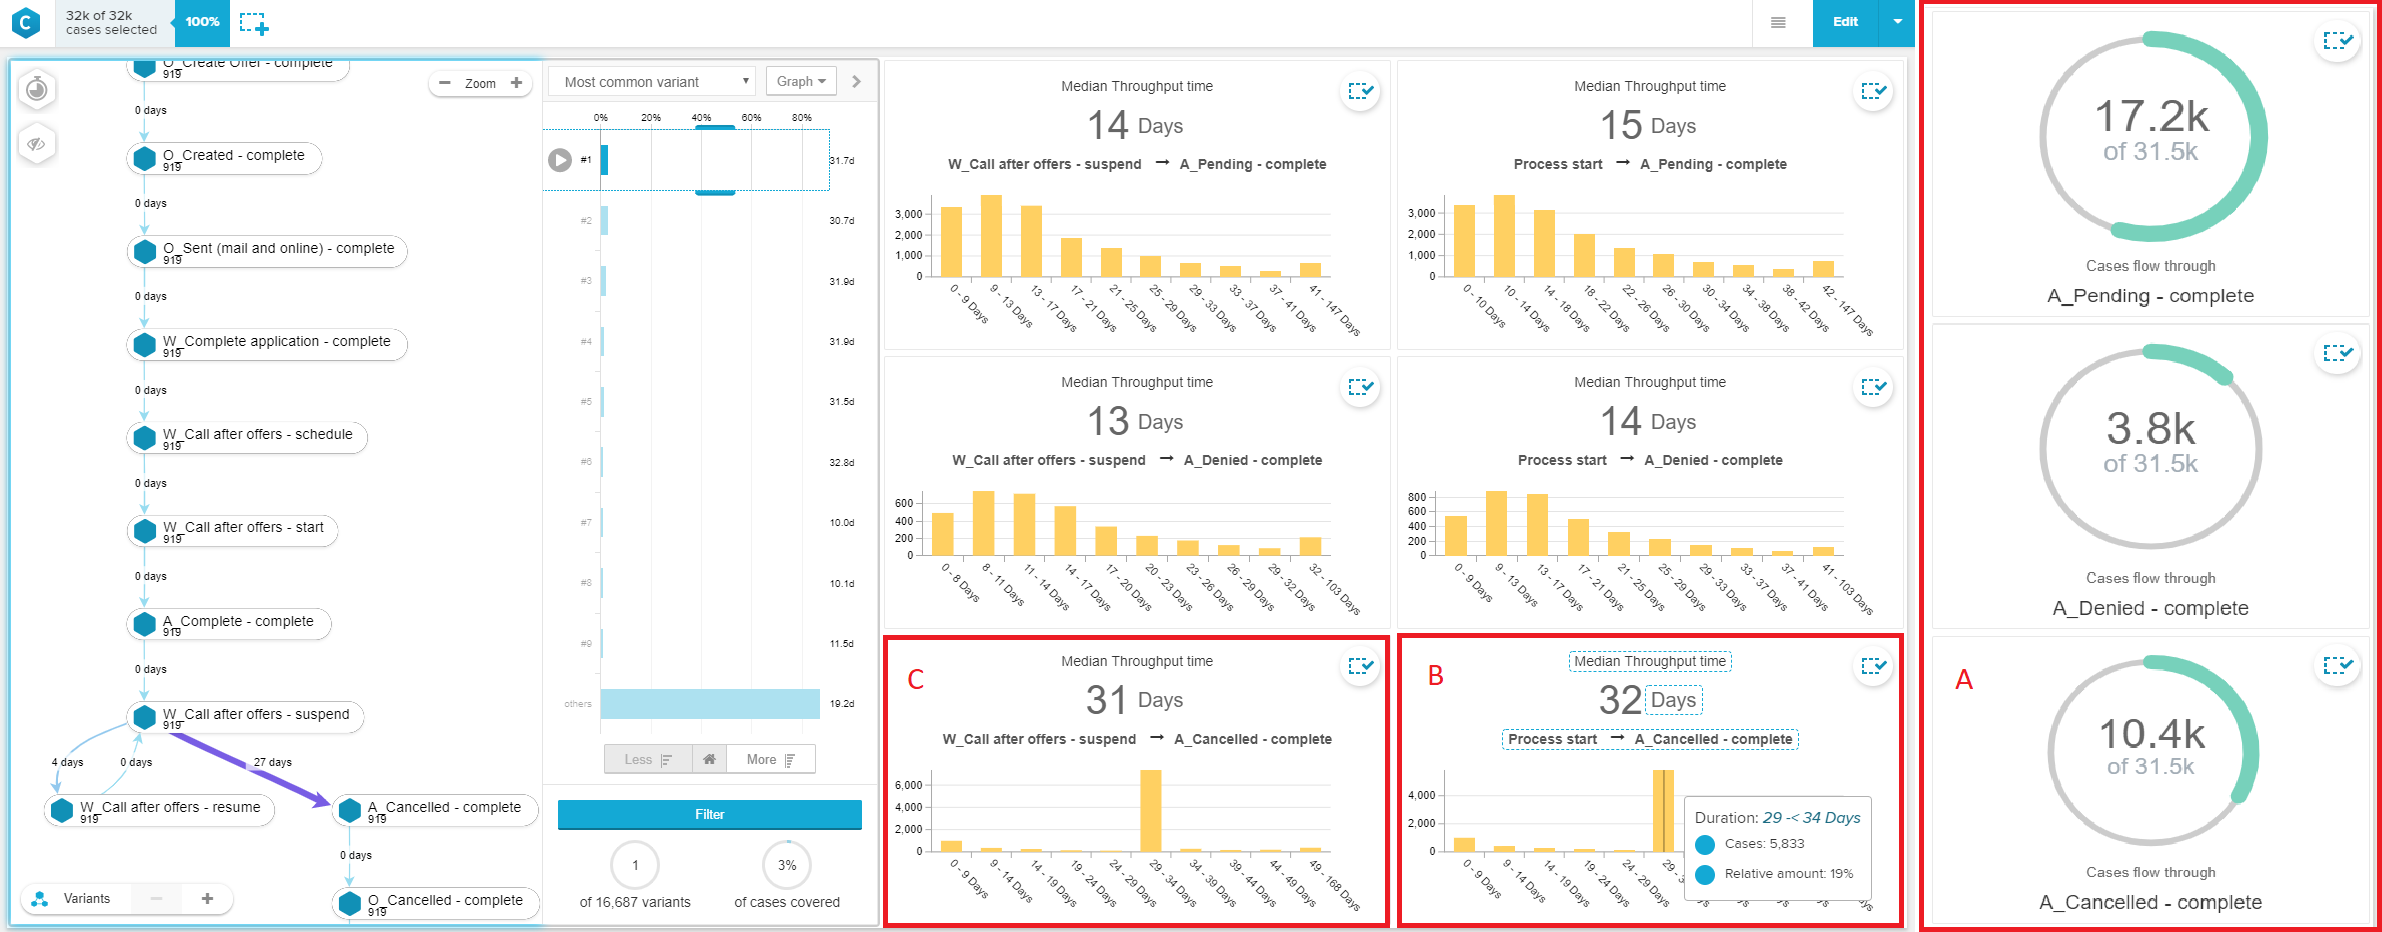
\includegraphics[width=0.25\textwidth]{images/throughput_time.png}
%\end{wrapfigure}

Our derivation affirms such questions by the financial institute about the interaction with the client and the fact of bottlenecks occurred also by the client.
Another view is equally put by the winner of the challenge\cite{winner} by dividing process flow into intervals. The process lag by client’s fault and the process lag by employee’s fault.




\section{Pre-processing log}

After over-viewing the whole process log by mining specific information within perspectives, and having some insights about what the critical parts of data to process could be, we aim to pre-process data as follows:
We use ProM platform to export XES file to CSV file to easy elaborate dataset in python environment to apply data mining techniques and further analysis.
The first step composed of cleaning log from incomplete cases since the log has been slipped in a point of time that there were some cases in phase of treatment.
(however, this step could be performed by ProM itself) but we want to assume that the final activity to consider in a case, this with one of outcome event (A\_Pending, A\_Cancelled or A\_Denied). To do so we cut case until these three events. It is important o notice the difference between to structures of log XES and CSV. XES is life cycle aware but csv is flat structure.
\begin{center}
\begin{table}[h]
\begin{tabular}{ l|c|c } 
 
 Log & Number of cases & Number of variants \\
 \hline
 Original & 31,509 & 4,047 \\ 
 
 Preprocessed & 31,194 & 3,544 \\ 


\end{tabular}
\caption{Original vs Pre-processed Log.\label{preprocessed}}\\
\end{table}
\end{center}

We find that there are 2,924 variant that contain only one case each, this make clustering methods challenging because each of these cases must -in the ideal way- considered as a unique cluster. In the other hand a cluster with one instance (case) will be non-useful and as this disadvantage we so call them difficult cases.





